\documentclass{article}
\usepackage{graphicx}
\usepackage{hyperref}

\begin{document}

\title{The HypeDyn 2 Hypertext Fiction Editor\\Tutorial 2: Fragments with Multiple Rules, Conditional Text and Anywhere Nodes}
% \author{Alex Mitchell}
\date{}

\onecolumn
\maketitle

\tableofcontents


\section{Introduction}
In this tutorial, we will introduce some new features to HypeDyn 2:

\begin{itemize}
  \item fragments with \textit{multiple rules}, which allows for different actions to be taken depending on which conditions are satisfied;
  \item \textit{conditional text}, which can be displayed \textit{instead of} the original text in a fragment; and 
  \item \textit{anywhere nodes}, which are nodes that can be automatically linked to from \textit{any} other nodes in the story based on conditions.
\end{itemize}

In this tutorial, we will be creating a variation of the ``Little Red Riding Hood'' hypertext fiction which you created in tutorial 1. We will change the story such that the reader is able to choose whether Red is naive or street-smart, which will have consequences as to how the story ends, and will also cause some of the text in the story to change. We will also add a ``summary'' node, reachable from all other nodes, which shows an up-to-date summary of the story so far.

\begin{figure}[h]
  \centering
  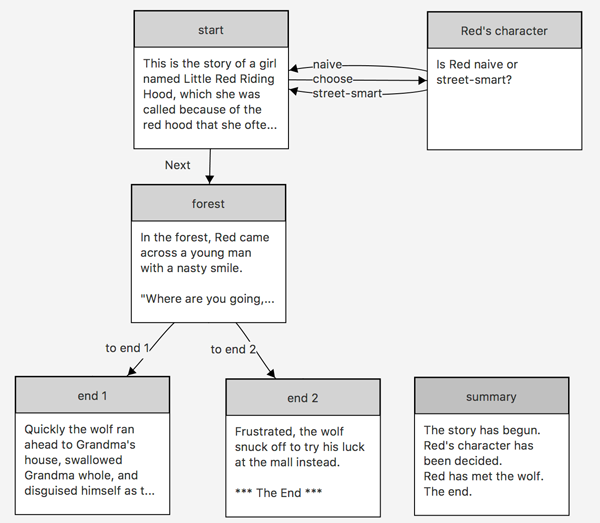
\includegraphics[width=11cm]{images/hypedyn-tutorial-2-figure-1}
  \caption{\textit{The completed ``Little Red Riding Hood'' story.}}
  \label{fig:tut2:completed}
\end{figure} 

The nodes and links in the final story are shown in Figure \ref{fig:tut2:completed}.

\textit{Note:  HypeDyn is a work-in-progress. If you encounter any errors, please report them as issues on our Github site: \url{https://github.com/narrativeandplay/hypedyn2}.}

\section{Getting started}

First, open HypeDyn by double-clicking on the file \textbf{HypeDyn2.exe} (in Windows) or \textbf{HypeDyn 2.app} (in MacOS).

We will continue from the story that you created in tutorial 1. If you don't have the story, you can start from the file \textsc{LRRH.dyn2} in the \textsc{examples} folder. HypeDyn files always end with a \textbf{.dyn2} extension.

%\textit{Note: for users of HypeDyn 1, the HypeDyn 2 file format is different from the HypeDyn 1 file format. If you have your LRRH.dyn file from the HypeDyn tutorial, you will not be able to load it in HypeDyn 2.}

We no longer need the ``Hood details'' node, so delete this node by clicking on the node in the map view on the right of the main window, and then clicking the ``Delete node'' button. Then go into the ``start'' node, and delete the fragment ``more about the hood'' which previously linked to the ``Hood details'' node by clicking on the ``-'' (minus) button to the left of the fragment in the fragment list. Save the resulting file under a different name.

\section{Fragments with multiple rules}

The first new feature we will introduce is the use of multiple rules on a fragment. This feature allows you to have different sets of actions which will be triggered when different conditions are satisfied.

For our story, we want to provide two different endings: one ending if Red is naive, and a second ending if she is street-smart. We will provide one fragment for the reader to click on and, depending on the choice that the reader made at the start of the story, the fragment will link to either the first or the second ending.

\subsection{Letting the reader make a choice}

To let the reader make a choice, we will create a node named ``Red's character'', which contains two fragments, one named ``naive'' and another named ``street-smart''. Both fragments link back to the start node. HypeDyn will keep track of which link was followed. Later in the story, we can check which of these two fragments the reader chose, and use this to make a decision. We will do this by creating a rule on the
``to the end'' fragment in the ``forest'' node which leads to node ``end1'' if link ``naive'' was followed, and a second rule which goes to node ``end2'' if link ``street-smart'' was followed.

Now we will create the node ``Red's character'' to let the reader make a
choice.

\begin{enumerate}
  \item Create a new node named ``Red's character''. In the new node, enter the following text:

\begin{quotation}
\noindent Is Red naive or street-smart?
\end{quotation}

\item Make a fragment on the text ``naive'', and name the fragment ``naive''.

\item Create one rule in the fragment, and also name the rule ``naive''.

\item Add an action to the fragment, so that clicking the fragment links to the ``start'' node.

\item Similarly, create a fragment on the text ``street-smart'', name the fragment ``street-smart'', and create a rule named ``street-smart'' that links back to the ``start'' node.

\item Note that changes made in the Node Editor are not actually applied to the story until you click the ``Apply'' button. If you look at the Map View now, you'll see that the new node is not visible. Now click on the ``Apply'' button to make these changes. The new node, and the two links you just created, will now be visible.

\item Recall that the rule contains a list of conditions (initially empty), plus a list of actions. The actions will be performed if the conditions are satisfied.

Since we don't want the reader to be able to change their choice, we will put a condition on the ``naive'' fragment: the link can only be followed if the reader \textit{hasn't} followed both the link ``naive'' and the link ``street-smart''. Do this by adding 2 conditions to the ``naive'' rule, as shown in Figure \ref{fig:tut2:red_is_naive}.

\begin{figure}[h]
  \centering
  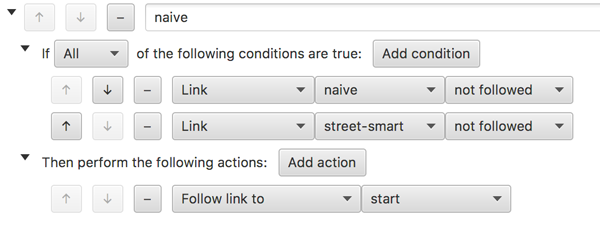
\includegraphics[width=10cm]{images/hypedyn-tutorial-2-figure-2}
  \caption{\textit{Adding conditions on the rule ``naive''.}}
  \label{fig:tut2:red_is_naive}
\end{figure} 

\noindent Make sure that you change the pulldown menu to the right of ``If'' to show \textit{All}. This tells HypeDyn that \textit{all} of the conditions must be satisfied. The other option, \textit{Any}, tells HypeDyn to perform the actions if \textit{at least one} of the conditions is satisfied. We will use the \textit{Any} option later in the tutorial.

\noindent In Tutorial 1, we used conditions which checked whether or not a \textit{node} had been \textit{visited}. Here, we are using conditions to check whether or not a \textit{link} has been \textit{followed}. HypeDyn also provides conditions which can check the state of \textit{facts}. We will cover facts in Tutorial 3.

\item Do the same to add conditions to the ``street-smart'' fragment.

\item Finally, edit the node ``start'', and make a link from the text ``Little Red Riding Hood'' to the node ``Red's character''. Name both the fragment and rule ``Red's character''. We don't want the reader to be able to go into ``Red's Character'' if they have already made a choice, so create the same conditions on this link as you did on ``naive'' and ``street-smart''.

\noindent Note that even though we put this condition on the link to ``Red's character'', we still need the conditions on the two links in the ``Red's character'' node, just in case the reader presses the \textit{back} button and tries to change their choice. Also, we can't just check whether or not the reader has visited the node ``Red's character'', as they may not have actually made a choice, just visited the node and then pressed \textit{back}.
\end{enumerate}

Now we have the mechanism in place to let the reader choose what sort of person Red is: naive or street-smart. We can check which of the two links were followed, ``naive'' or ``street-smart'', whenever we want to make a decision which is influenced by Red's character. This is an example of using the \textit{followed state} of a link as a way of representing some information about the state of the storyworld. Similarly, we could use the \textit{visited state} of a node to represent some information. This is a very useful technique which can be generalized to allow for more complex, dynamic behaviour.

% need to explain 1) that the label on the link is the name of the rule, and 2) that the check is against the fragment being activated, so the name in the pull-down is the fragment name, not the rule name...

\subsection{Following a link based on the reader's choice}

Now we will create the link to the two different endings, and set up the rules so that the reader will follow the link to the appropriate ending based on the reader's \textit{earlier} choice about Red's character.

\begin{enumerate}
  \item First, rename the current ``end'' node to ``end 1'' by editing the node in the Map view, and changing the name in the ``Name'' text field.
  \item Still editing the node ``end 1'', delete the text ``back to start''. Notice that the fragment ``restart'' attached to the text ``start'' is deleted when you delete the text. If you apply the change by clicking on the ``Apply'' button, you will see the link also disappears from the Map View.
  \item Next, replace the text in the node ``end 1'' with the following text:
  \begin{quotation}
  \noindent Quickly the wolf ran ahead to Grandma's house, swallowed Grandma whole, and disguised himself as the poor old lady. When Red arrived, he finished her off too. Yum!
  
  \bigskip
  
  \noindent *** The End ***
  \end{quotation}
  \item Now create a new node, named ``end 2'', and enter the following text:
  \begin{quotation}
  \noindent Frustrated, the wolf snuck off to try his luck at the mall instead.
  
  \bigskip
  
  \noindent *** The End ***
  \end{quotation}

\item Now that we have the two endings in place, we need to make sure that the link from the text ``next'' in node ``forest'' takes the reader to ``end 1'' if Red is naive. Otherwise (ie. if Red is street-smart), the link should take the reader to ``end 2''. To do this, we will add conditions to the current rule, and then add a second rule to the ``to the end'' link.

Edit the ``to the end'' link on the text ``next'' in node ``forest''.
The original link, from the previous version of the story, has a single rule, ``to the end'', which has no conditions and contains a single ``follow link to'' action, leading to the original end node, now renamed ``end 1''.

\item We are doing to change this rule so that it only takes the reader to ``end 1'' if Red is naive. To help us remember this, we can rename the rule to reflect what it does. Rename the rule as ``to end 1''. This is the label which will appear in the Map view.

\item Now add a condition that link ``naive'' is followed (see Figure
\ref{fig:tut2:to_end_1}).

\begin{figure}[h]
  \centering
  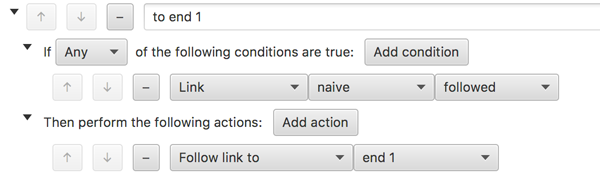
\includegraphics[width=10cm]{images/hypedyn-tutorial-2-figure-3}
  \caption{\textit{Condition on the rule leading to ``end 1''.}}
  \label{fig:tut2:to_end_1}
\end{figure}

\item This gives us the required behaviour for a naive Red. However, if the conditions are \textit{not} satisfied, ie. if Red is street-smart, clicking on the fragment won't go anywhere. Next we need to use the same fragment, but now specify what should happen in this case. To do this, we will create a second rule.

Add a second rule by clicking on the ``Add Rule'' button. You should now
see a second rule beneath the ``to end 1'' rule, named ``new rule''  (see Figure \ref{fig:tut2:new_rule}).

\begin{figure}[h]
  \centering
  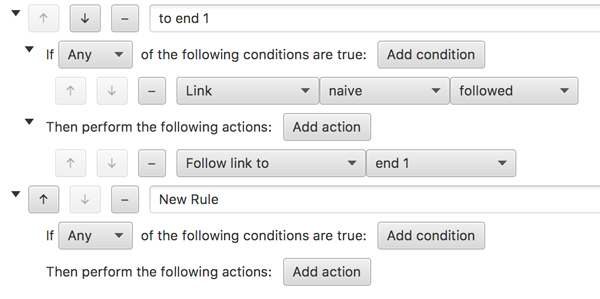
\includegraphics[width=10cm]{images/hypedyn-tutorial-2-figure-4}
  \caption{\textit{Adding a second rule.}}
  \label{fig:tut2:new_rule}
\end{figure}

Note that if you find that the rule list is becoming too cluttered, you can \textit{collapse} rules by clicking on the small triangle at the left of the rule. This hides everything except the the first line of the rule. Click the triangle again to \textit{expand} the rule.

\item Change the name of the new rule to ``to end 2''. This will remind us that this rule contains the action to follow the link to ``end 2''.

\item Add a ``follow link to'' action, and set its pulldown menu to ``end 2''.

\item At this point, we have two rules, one which leads to ``end 1'' if the link ``naive'' was followed, and the other which always leads to ``end 2''. This is not quite right -- what will happen if you try reading the story now? First try choosing Red's character to be naive, and then restart the story and try making her street-smart.

As you will have noticed, the link always goes to ``end 2'', whichever link you choose in ``Red's character''. To understand why this is, we need to look at how HypeDyn evaluates rules.

When the reader clicks on a link, HypeDyn looks at the rules in a link one by one, from the top of the list of rules. For each rule, it determines whether the conditions are satisfied. If the conditions are \textit{not} satisfied, it goes to the next rule, and again checks this rule's conditions. It keeps doing this until it finds a rule for which the conditions are satisfied. Once this happens, it carries out the actions in that rule.

After the actions have been carried out, HypeDyn looks to see whether or not the ``Stop if true'' option has been checked for the current rule. If it has been checked, then it stops. Otherwise, it continues on to the next rule, and repeats the process of checking conditions and carrying out actions.

So in our case, HypeDyn first looks at the ``to end 1'' rule. In the case where the reader has chosen ``street-smart'', HypeDyn will check the conditions for ``to end 1'', see that they are not satisfied, and then move on to the second rule. Since there are no conditions on the second rule, HypeDyn carries out its actions, taking the reader to node ``end 2''. This is what we want.

If the ``naive'' link has been followed, HypeDyn checks the conditions for the ``to end 1'' rule, sees that they \textit{are} satisfies, and carries out the action, taking the reader to node ``end 1''. It then looks at the ``Stop if true'' option, which is not checked, and moves on to the second rule, ``to end 2''. Since there are no conditions on the second rule, HypeDyn carries out its actions, taking the reader to node ``end 2''. This is \textit{not} what we want!

\item To fix this, the easiest solution is to check the ``Stop if true'' option on the ``to end 1'' rule. This will tell HypeDyn not to continue to the next rule if the first rule has been satisfied. Do this now (see Figure \ref{fig:tut2:rules_with_stop}).

\begin{figure}[h]
  \centering
  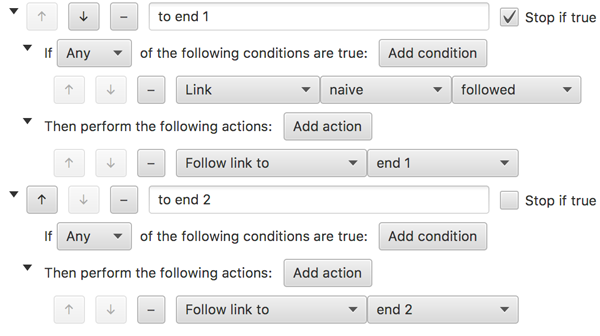
\includegraphics[width=10cm]{images/hypedyn-tutorial-2-figure-6}
  \caption{\textit{Stopping if the first rule is satisfied.}}
  \label{fig:tut2:rules_with_stop}
\end{figure}

\item Now try running the story again. It should behave as we intended -- if the we choose that Red is naive, we will see the first ending, and if we choose that she is street-smart, we will see the second ending.

\end{enumerate}

Note that there is another way to fix this problem. Instead of checking the ``Stop if true'' option on the ``to end 1'' rule, we could have put a condition on the ``to end 2'' rule stating that the rule's actions should only be carried out if the ``street-smart'' link was followed. However, this would mean that every time the reader chooses the ``naive'' link, the second rule's conditions are checked. For such a simple rule this is not a problem, but if the rule becomes more complex, this can slow down your story.

\subsection{Forcing the reader to make a choice}

At this point we seem to have everything in place for the reader to make a choice which impacts the end of the story. However, with our current
implementation, if the reader ignores the link on the text ``Little Red Riding Hood'' in the ``start'' node, and goes through to the end of the story, she will always end up with the second ending.

To fix this, we need to force the reader to make the choice about Red's character \textit{before} we let her move on to the ``forest'' node. We can do this by putting a condition on the link from ``start'' to ``forest'' such that the link can only be followed if \textit{either} link ``naive'' \textit{or} link ``street-smart'' have been followed.

\begin{enumerate}
  \item Edit the rule ``Next'' in the link ``Next'' in node ``start''.
  \item Add the following condition: link ``naive'' was followed.
  \item Add the following condition: link ``street-smart'' was followed.
  \item Now change the pulldown menu to the right of ``IF'' to show ``Any'' (see Figure \ref{fig:tut2:any_condition}).

\begin{figure}[h]
  \centering
  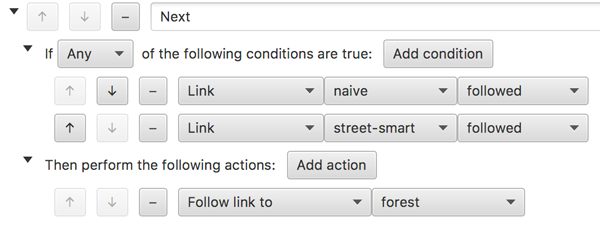
\includegraphics[width=10cm]{images/hypedyn-tutorial-2-figure-7}
  \caption{\textit{Specifying two conditions where \textbf{any} can be
  satisfied.}}
  \label{fig:tut2:any_condition}
\end{figure} 

This means that the link will be followed if \textit{at least one} of the listed conditions are satisfied, which is what we want.

\end{enumerate}

\subsection{Testing the story}

Now that we have our story in place, we can test the story. You can do this by clicking the \textit{Run} button. The \textit{Run} button will read the story starting at the node which was set as the \textit{start} node.

Try clicking through the story. You should be able to choose Red's character, and then see a different ending based on your choice. You can stop reading by closing the browser window.

\section{Specifying conditional text}

As you read through the story, you probably realized that there's a problem: the story doesn't really make sense. There's no explanation as to why the wolf was unable to eat Red if she's street-smart. It also doesn't seem reasonable that, as a street-smart little girl, she would have told the wolf that she was going to Grandma's house.

So, it would be good if we could change what Red says to the wolf depending on what choice the reader made regarding Red's character. This is where \textit{conditional text} is useful.

What we want to do is set a condition so that, if the reader has chosen for Red to be street-smart, the text ``I'm off to see my sick granny'' in the ``forest'' node will automatically be changed to ``I'm not supposed to talk to strangers.''

\begin{enumerate}
  \item Edit the node ``forest''.
  \item Select the text ``I'm off to see my sick granny'', and click on
  ``Add fragment''. Name the fragment ``response''.
  \item Create a new rule, and name it ``street-smart''.
  \item Add a condition, and set the following condition: link ``street-smart'' is followed.
  \item Now add an action, and choose action type ``Update fragment text''. Make sure the action's pulldown menu reads ``Input'', and type the following text into the action's text field (see Figure \ref{fig:tut2:alttext}):
  \begin{quotation}
  \noindent ``I'm not supposed to talk to strangers.''
  \end{quotation}

\begin{figure}[h]
  \centering
  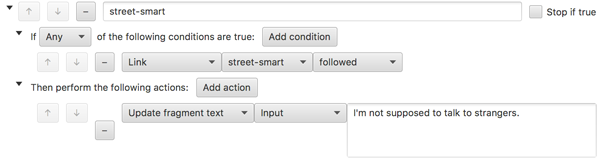
\includegraphics[width=12cm]{images/hypedyn-tutorial-2-figure-8}
  \caption{\textit{Specifying alternative text.}}
  \label{fig:tut2:alttext}
\end{figure} 

Since we don't want the reader to actually be able to click on this fragment, we won't add a ``follow link to'' action. Without a ``follow link to'' action, the fragment will not be underlined or bold when you read the story.
  \item Click on ``ok'' to close the \textit{Edit node} window.
\end{enumerate}

That's it! Now test the story by clicking on the ``Run'' button. You should see the appropriate text in the ``forest'' node, depending on which personality you chose for Red. If you choose ``naive'', the condition is not satisfied, the action is not performed, and you see the original text. If, instead, you choose ``street-smart'', the condition is satisfied, and the text is replaced by the text you entered in the ``Update fragment text'' action.

This is a simple feature, but it is a major addition to what can be done in HypeDyn. Text is no longer fixed - the author can procedurally alter/generate text within a node, based on the reader's actions. 

Note that we could get the same effect (from the reader's perspective) by
creating 2 nodes -- one with the original text, and one with the ``street-smart'' text. This is a reasonable solution when there is one change, such as in our simple story for this tutorial. However, if there are many nodes which need to be changed based on the choice of Red's character, it will quickly become difficult for the author to keep track of the text. It gets even more complicated if there are is than one choice that the reader can make. Using conditional text is a much more appropriate and manageable approach.

\section{Anywhere nodes}

The last thing we are going to do is to add in an \textit{anywhere} node. This is a node which is automatically linked from all the nodes in the story. This feature is useful as a way to create, for example, a summary of the story so far, or a list of the decisions that the reader has made. 

\subsection{Adding the anywhere node}
In our case, we will create a summary of the story so far using an anywhere node.

\begin{enumerate}
  \item Click on ``New node'', and name the new node ``summary''. 
  \item Now edit the node, and click on the \textit{Node rules} tab in the rules list. This shows the list of node rules, rules that apply to the \textit{entire node} rather than to a specific fragment.
  \item Create a new rule, and name the rule ``Anywhere node''.
  \item Add the action \textit{Enable anywhere link to here} (see Figure \ref{fig:tut2:anywherenode}).

\begin{figure}[h]
  \centering
  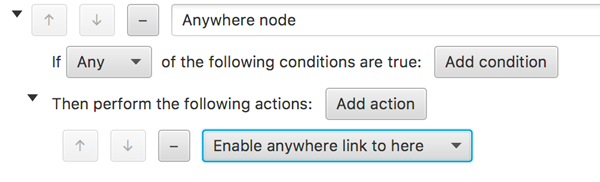
\includegraphics[width=10cm]{images/hypedyn-tutorial-2-figure-9}
  \caption{\textit{Creating an anywhere node.}}
  \label{fig:tut2:anywherenode}
\end{figure} 

\noindent Now close the Edit Node window. Notice that background behind the name of the new node is a darker grey that regular nodes. The difference in colour is used to indicate anywhere nodes. An anywhere node is almost the same as a regular node, with the exception of a special action that we added to the ``node rules''. Removing this action turns an anywhere node back into a regular node. We will discuss node rules in detail in Tutorial 3.

  \item Edit the node by selecting it and clicking on ``Edit node'', as with a regular node.

  \item In the node, enter the following text:
  \begin{quotation}
  \noindent The story has begun.
  
  \bigskip
  
  \noindent Red's character has been decided.

  \bigskip

  \noindent Red has met the wolf.

  \bigskip

  \noindent The end.
  \end{quotation}
\end{enumerate}

If you run the story now, you will see a link with the text ``summary'' has been added to the bottom of every node. Clicking on this link will take you to the node which we just created.

\subsection{Adding some conditional text}
We want the second line to be displayed only after the reader has decided on Red's character, the third line after the ``forest'' node has been visited, and the last line once the reader has reached the end of the story. We can do this using conditional text, as shown in the previous section.

\begin{enumerate}
  \item Select the second line of text, and click on ``Add fragment''. Name the fragment ``character''.
  \item Create a new rule, and also name it ``character''.
  \item We want the text in this fragment to only be shown after the reader has decided on Red's character. So first what we need to do is create an action to \textit{remove} the text when the reader has \textit{not} yet decided on Red's character. Add an ``Update fragment text'' action, select ``Input'', and leave the text blank. This will blank out the fragment's text when this rule's conditions are met.
  
  \item Now we want to set the conditions for when the text is blanked. Since we want the first line to show \textit{after} the reader has chosen Red's character, we need two conditions: the link ``naive'' has \textit{not} been followed, and the link ``street-smart'' has \textit{not} been followed. Add these two conditions.
  \item Since we want the text to show when \textit{both} of these links have not been followed, make sure the the type of the rule is set to ``All''.
\end{enumerate}

\subsection{Adding the remaining conditional text}
Now do the same for the third and final lines:

\begin{enumerate}
  \item Add a fragment, named ``forest'', on the third line.
  \item Add a rule, also named ``forest'', to the ``forest'' fragment.
  \item Add one condition, that the ``forest'' node has not been visited.
  \item Add an ``Update fragment text'' action, select ``Input'', and leave the text blank.
  \item Add a fragment, named ``end'', on the final line.
  \item Create a rule, and also name it ``end''.
  \item Add two conditions, that the ``end 1'' node has \textit{not} been
  visited, and that the ``end 2'' node has \textit{not} been visited.
  \item Finally, add an ``Update fragment text'' action, select ``Input'', and leave the text blank.
\end{enumerate}

This completes the ``summary'' node. Close the node, Try running the story, and go through the two story. There should now be a ``summary'' link at the bottom of all regular nodes. If you click on the link, you should see a node with the summary of the story. The text in the summary node should gradually be revealed as you move through the story.

\section{Next steps}

We have created a simple story, with a choice at the start which changes what happens in the story, including the ending. The completed version of this story can be found in the file \textsc{LRRH2.dyn2}.

There are several things that you could try to enhance the story. For example, you could change the description of Red in the ``start'' node, depending on whether she is naive or street-smart. You could also customize the summary of the story depending on which personality the reader chose. One way of adding these enhancements can be found in \textsc{LRRH3.dyn2}.

\section{Conclusion}

In this tutorial, we have created a simple hypertext fiction which includes a choice for the reader regarding Red Riding Hood's character. We have seen how to make use of multiple rules and conditional text to adapt the story to the reader's choice. This functionality provides the basis for moving away from stories which make use of predetermined content and branches, towards more procedural hypertext. In tutorial 3, we explore more extensive use of procedural hypertext, introducing ``node rules'' and ``facts''.

\end{document}
